%\clearpage
%//==============================--@--==============================//%
\subsection{P2 | Efeito do fármaco em função da dose (modelo PD)}
\label{subsec:P2}

A farmacodinâmica (PD) permite descrever a relação\footnotemark[2] entre o efeito de um fármaco ($u$) e a sua concentração ($C_p$) no compartimento de efeito. O modelo PD é amplamente representado pela equação de Hill\cite{Goutelle2008-bv}:

\vspace{-1em}
\begin{equation}\label{eq:modelo-PD}
    u \delequal u_{max}\frac{C^\alpha_p(t)}{C^\alpha_{50} + C^\alpha_p(t)}
\end{equation}
onde $u_{max}$ é o efeito máximo do fármaco (tipicamente um valor unitário\cite{teles_2017}), $C_{50}$ a concentração para qual 50\% do efeito máximo é obtido\footnotemark[3], e $\alpha$ denota o coeficiente de Hill que determina a \textit{steepness} da sigmoide resultante.
%//==============================--@--==============================//%
\footnotetext[2]{Contribui para a compreensão da resposta medicamentosa e da sua eficácia.}
\footnotetext[3]{Considera-se $C_{50} = 7.1903$ mg/kg (Atezolizumab)\protect\cite{belfo_2018}\cite{teles_2017}.}
%//==============================--@--==============================//%
\newpage
\vskip -1em
\begin{wrapfigure}{l}{0.5\textwidth}
    \centering
    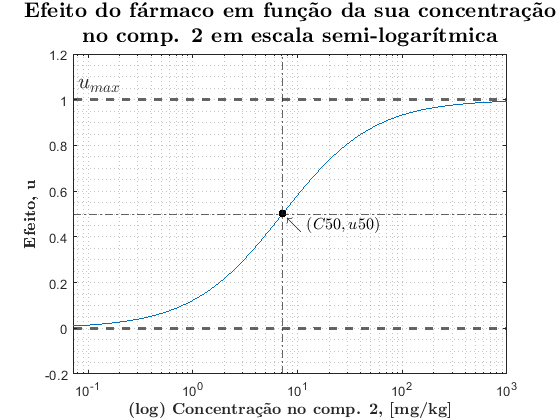
\includegraphics[width=0.5\textwidth]{img/perguntas/P2/P2-Hill.png}
    \caption{Efeito do fármaco em função de $C_p$ em escala semi-logarítmica\protect\footnotemark[4] (com os níveis de saturação salientados), para $\alpha = 1$, $u_{max} = 1$ e $C_{50} = 7.1903$ ($\pmb{\star}$ \textbf{valores considerados ao longo do relatório}).}
    \label{fig:P2-Hill}
\end{wrapfigure}

Como explicitado na \hyperref[fig:P2-Hill]{Fig. 2}, a equação de Hill introduz uma saturação na variação da concentração do fármaco. 

Tal traduz-se em concentrações baixas, resultarem em efeitos bastante diminutos; e concentrações elevadas, tenderem para um efeito saturado, i.e., $\pmb{\star}$ \textbf{administrações com dosagens \underline{mais elevadas} do que um certo patamar, \underline{não produzem} um maior efeito na redução do tumor}.

Para além disto, há que ter em consideração a carga tóxica a que o organismo é exposto na terapia, o que torna a dosagem num parâmetro de fulcral controlo, proeminentemente com fármacos de elevada toxicidade. Acrescenta-se:

\vphantom{Experiência 123}

\vspace{-1.5em}
\begin{quote}
    ``\textit{O que é que não é um veneno? Todas as coisas são veneno e nada é sem veneno. Somente a dose determina que algo não seja um veneno.}''
    
    \attrib{Paracelso}
\end{quote}

\vspace{-1.5em}
\begin{wrapfigure}[16]{l}{0.5\textwidth}
    \centering
    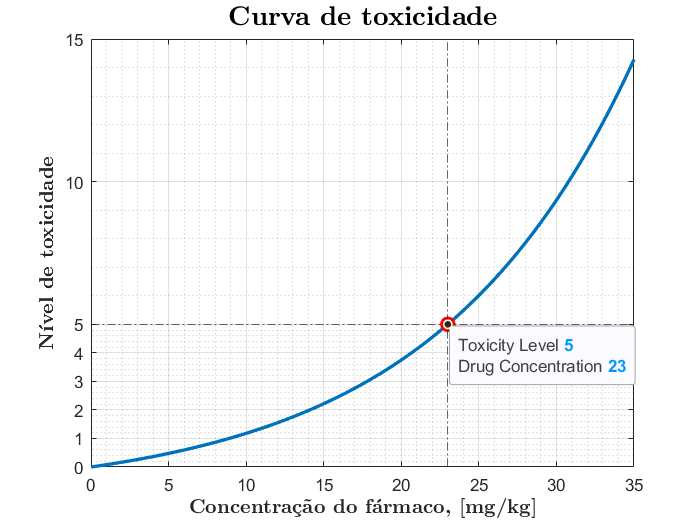
\includegraphics[width=0.5\textwidth]{img/perguntas/P2/P2-toxicity.png}
    \caption{Níveis de toxicidade para o fármaco Atezolizumab. A marca representa a concentração para qual o nível de toxicidade é máximo (\textit{grade} 5).}
    \label{fig:P2-toxicity}
\end{wrapfigure}

\vphantom{1}
\vskip 0.25em
No entanto, os níveis de toxicidade não podem ser explicitamente aferidos\footnotemark[5] e não existem modelos para esta avaliação\cite{teles_2017}.

Ao estudar a concentração de um fármaco no organismo durante uma terapia, é possível estimar os níveis de toxicidade ``\textit{by using a function yielding a certain small value until a certain amount of concentration is achieved. After this threshold, the function grows exponentially}\cite{toxicity-lemos}.''\cite{teles_2017} A \hyperref[fig:P2-toxicity]{curva de toxicidade} foi escolhida de modo a que a \textit{morte}\footnotemark[5] seja atingida quando a concentração do fármaco no organismo excede por 15\% o maior valor de dose permissível\footnotemark[6].
%//==============================--@--==============================//%
\footnotetext[4]{"The semi-log plot is the preferred method for plotting concentration-response relationships because it becomes easier to accurately determine the EC50 value (...) by placing it on a linear portion (...)"\cite{Salahudeen2017-pb}}

\footnotetext[5]{Não obstante, o \textit{Common Terminology Criteria for Adverse Events} (CTCAE) permite classificar a toxicidade em ensaios clínicos como:\\
$\xrightarrow[]{}$ leve (\textit{grade} 1), moderada (\textit{grade} 2), severa (\textit{grade} 3), risco de morte (\textit{grade} 4) e morte (\textit{grade} 5).}

\footnotetext[6]{Para o fármaco Atezolizumab $\xrightarrow[]{}$ 20 mg/kg\cite{Fu_undated-zm}.}